\documentclass{llncs}

\usepackage[utf8]{inputenc}
%\usepackage{fancyvrb,amssymb,graphicx}
%\usepackage[usenames,dvipsnames,svgnames,table]{xcolor}

% the following package is optional:
\usepackage{latexsym} 

\usepackage{graphicx}
% \usepackage{caption}
\usepackage{subcaption}
\captionsetup{compatibility=false}

\usepackage{wrapfig}

\usepackage{amsmath}
\usepackage{xspace}
\usepackage{graphicx,url}
\usepackage{txfonts} % needed for \Diamondblack
\usepackage{color}
\usepackage{xcolor}

%\usepackage{modallogics}
\newcommand{\logic}[1]{\textbf{#1}\xspace}
\newcommand{\KB}{\logic{KB}}
\newcommand{\KFour}{\logic{K4}}
\newcommand{\KFourB}{\logic{K4B}}
\newcommand{\K}{\logic{K}}
\newcommand{\KT}{\logic{KT}}
\newcommand{\SFour}{\logic{S4}}
\newcommand{\SFive}{\logic{S5}}
\newcommand{\SFiveU}{\logic{S5\textsuperscript{U}}}

\newcommand{\imp}{{\rightarrow}}
\newcommand{\biimp}{\leftrightarrow}
\newcommand{\allq}{\forall}
\newcommand{\exq}{\exists}
\newcommand{\seq}{\vdash}

\newcommand{\Dia}{\Diamond} % possibly
\newcommand{\BlackBox}{\blacksquare}
\newcommand{\BlackDia}{\Diamondblack}

\newcommand{\NE}{\mathit{NE}}
\newcommand{\ess}[2]{#1\ \mathit{ess}\ #2}
\newcommand{\nec}{\Box}
\newcommand{\pos}{\Dia}



\begin{document}

\title{An Object-Logic Explanation for the Inconsistency in G\"odel's Ontological Theory}
\author{Christoph Benzm\"uller\inst{1}\thanks{This work has been supported by
    the German Research Foundation DFG under grants BE2501/9-1,2} \and Bruno Woltzenlogel Paleo\inst{2} 
}

\institute{
 Freie Universit\"at Berlin, Berlin, Germany \\ \url{c.benzmueller@fu-berlin.de}
\and
 Australien National University, Canberra,  Australia \\ \url{bruno.wp@gmail.com}
}

\maketitle            



\begin{abstract}
  This paper discusses the discovery of the 
  inconsistency in G\"odel's
  ontological argument as a success story for artificial
  intelligence. Despite the popularity of G\"odel's argument, this
  inconsistency remained unnoticed until 2013, 
  when it was detected automatically by the 
  higher-order theorem prover \textsc{Leo-II} \cite{ECAI2014}. Complementing the meta-logic explanation for the inconsistency available in our IJCAI 2016 paper \cite{C55}, we present here a new purely object-logic explanation that does not rely on semantic argumentation.
  
  % (This extended abstract is mostly a shortened version of our IJCAI 2016 paper \cite{C55}, but the explanation of the inconsistency is more detailed here.)
\end{abstract}


% ToDo: Use \textsc for all system names


\section{Introduction}\label{sec:introduction}
% Without exaggeration 
Kurt G\"{o}del's ontological
argument for the existence of God \cite{GoedelNotes,ScottNotes} is
amongst the most discussed formal proofs in modern literature. A rich
body of publications -- including very recent ones -- present,
discuss, assess, criticize, modify and improve G\"{o}del's original
work (see e.g.~Sobel~\cite{sobel2004logic} and Oppy~\cite{sep-ontological-arguments} and the
references therein). 

Scott's version of G\"odel's argument was automatically reconstructed by the higher-order theorem prover \textsc{Leo-II} \cite{C40} and its correctness was verified step-by-step in the Coq proof assistant \cite{CSR}. To bridge the gap between higher-order logics (HOL; cf.~\cite{andrewsSEP} and the references
therein), as used by these systems, and higher-order \emph{modal} logics (HOML; cf.~\cite{homl} and the
references therein), on which the ontological argument argument, the logic embedding approach \cite{J23,C40} was used.

However, G\"odel's original axioms, as used in his
manuscript \cite{GoedelNotes}, are inconsistent. This fact has
remained unnoticed to philosophers until 2013, 
when \textsc{Leo-II} found a surprising refutation of the axioms.

In \cite{C55}, we have extracted from Leo-II's machine-oriented refutation an informal and human-oriented intuitive explanation for the inconsistency, and we have reconstructed and
verified it in the Isabelle proof assistant. However, that explanation relied on reasoning at the meta-logic (HOL) level, which was only possible because of the embedding. Here we complement that work with a purely object-logic (HOML) explanation.

Applications of (first-order) theorem proving technology in
metaphysics were first reported by Fitelson, Oppenheimer and
Zalta~\cite{FitelsonZalta,oppenheimer11}. 
%Zalta also coined the term
%\textit{Computational Metaphysics}. 
Later on, Rushby~\cite{rushby13} used the \textsc{PVS} proof
assistant. Common to both works is a
significant amount of proof-hand-coding work as well as their focus on
a non-modal formalization of St. Anselm's simpler
and older ontological argument.


\begin{figure}\centering 
  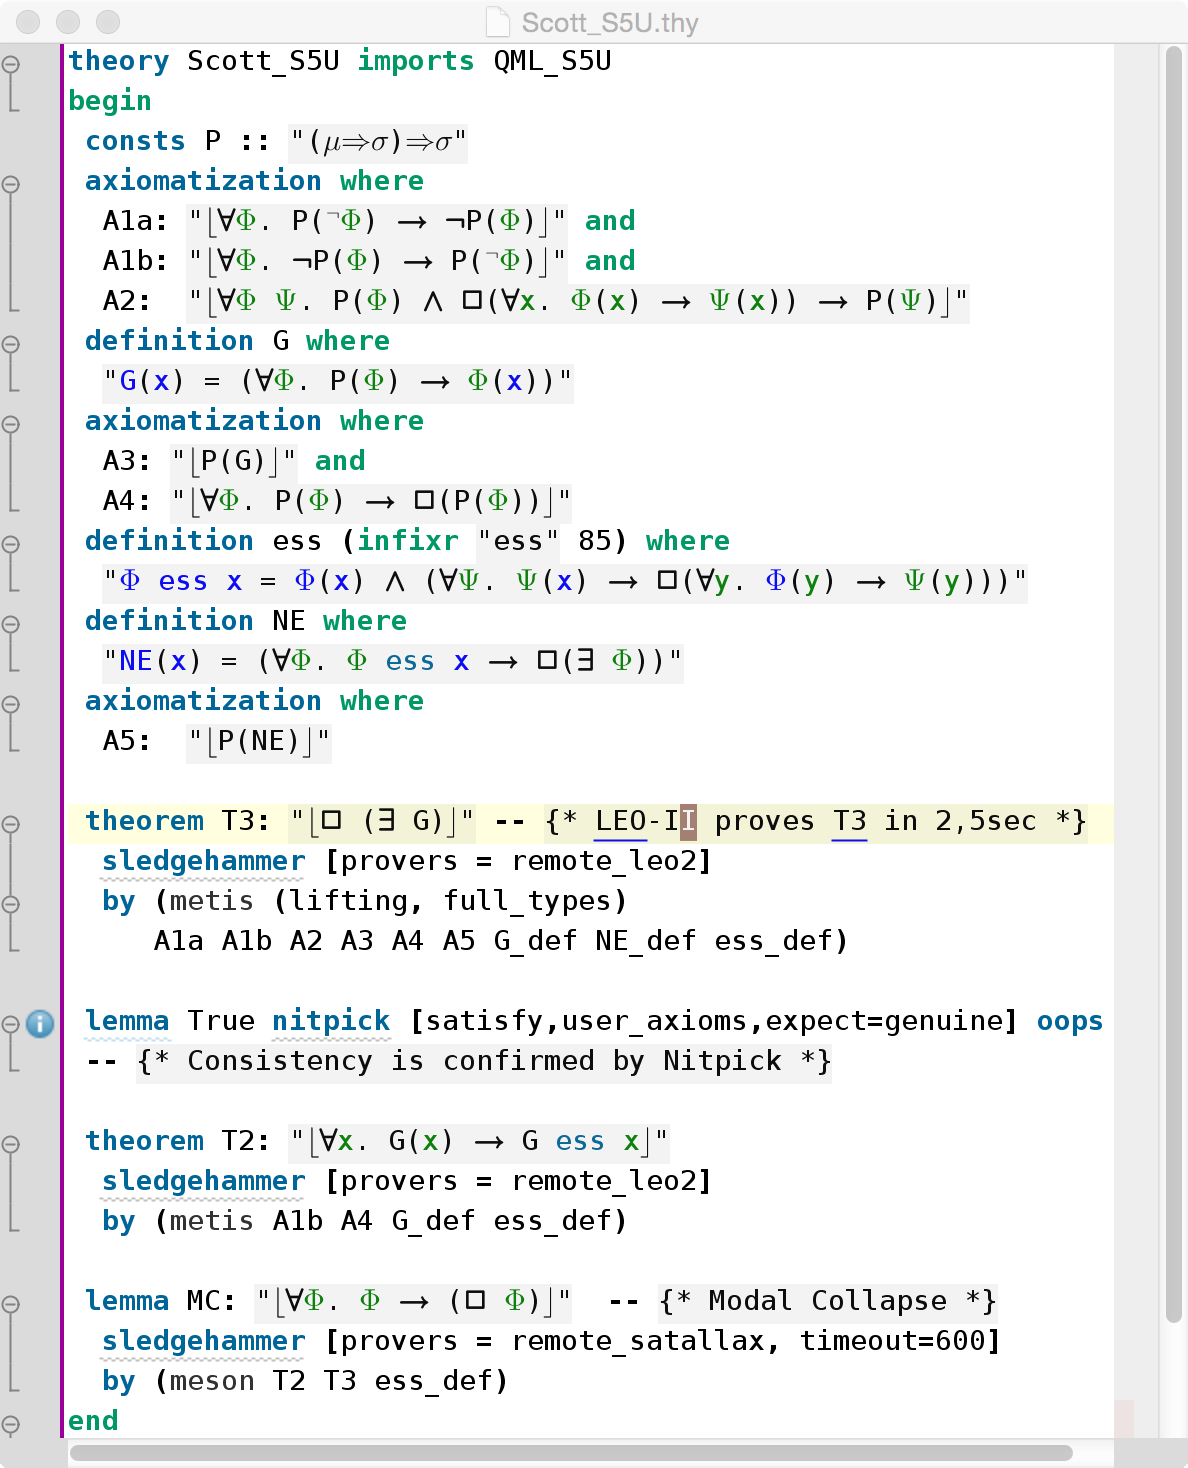
\includegraphics[width=.495\textwidth]{./Scott_S5U.png}
  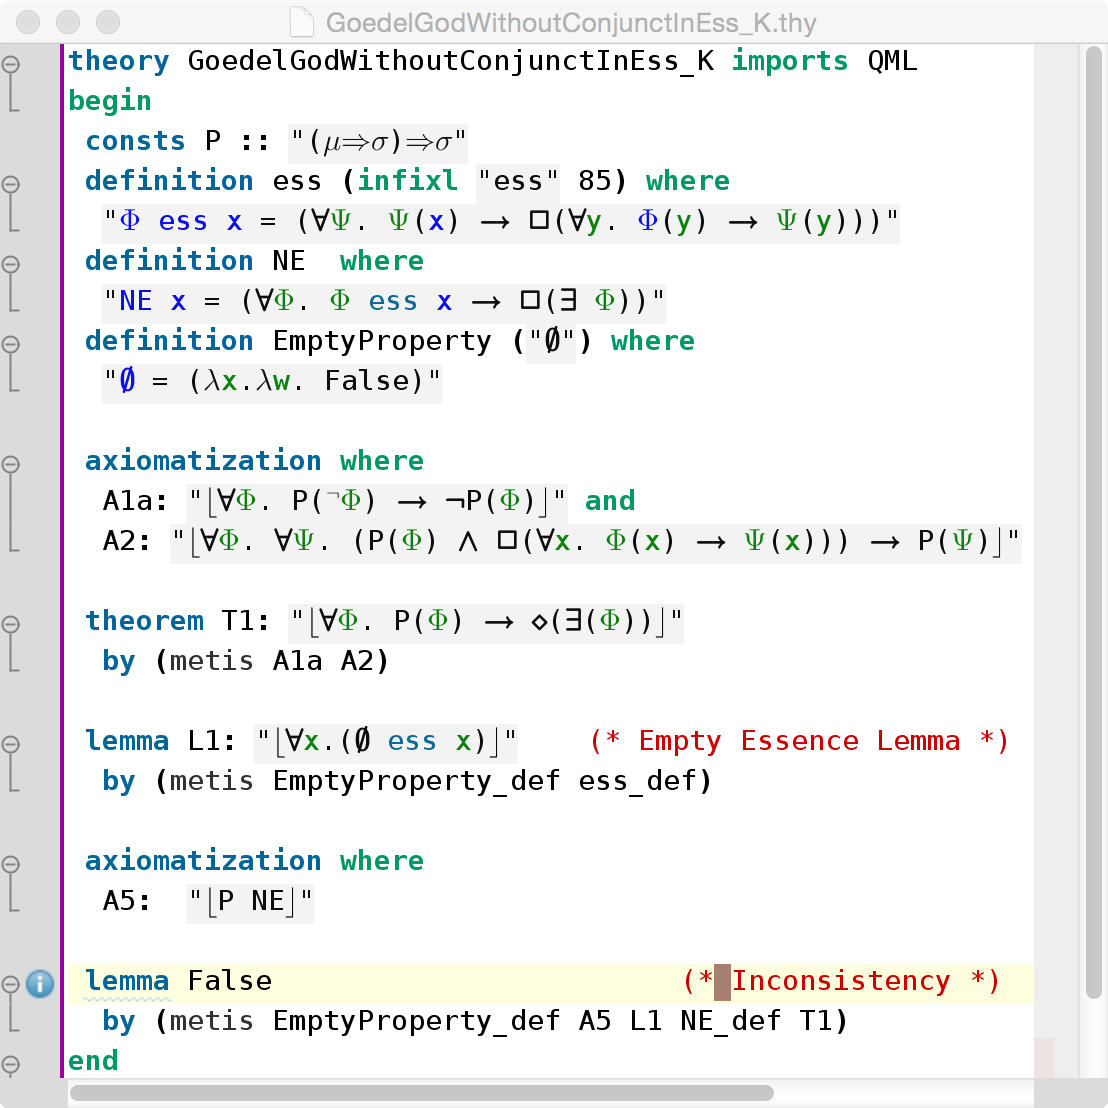
\includegraphics[width=.495\textwidth]{./InconsistencyIsabelleK.png}
  % \caption{Full Automation of T3 in \SFiveU; Consistency of Scott's
  % Axioms;  Automatic Verification of Modal Collapse} 
\caption{Scott's consistent axioms (left) and proof of the
  inconsistency of (a subset of) G\"odel's original  axioms (right)}
  % Axioms;  Automatic Verification of Modal Collapse} 
\label{Scott_Goedel}
\end{figure} 



\section{An Essential Difference in the Definitions of Essence.}
\label{sec:history}
G\"odel's manuscript can be considered a translation of Leibniz's
ideas on the argument into modern modal logic. G\"odel
discussed his manuscript with Scott, who shared a slightly different
version with a larger public. Scott's version of the axioms and
definitions, formalized in Isabelle, is shown in
Fig.~\ref{Scott_Goedel}. 
The main difference to G\"odel's version is an
extra conjunct in the definition of \emph{essence} (\emph{ess}). For Scott,
an essential property of an individual must be possessed by
him/her. For G\"odel, this is not required. 


G\"odel's omission has been
considered inessential and merely an oversight by many. 
For more than four decades, its serious consequences remained unnoticed, 
despite numerous analyses and criticisms of the
argument.
However, as explained here, the extra conjunct is in
fact crucial. Without it, G\"odel's original axioms are
inconsistent. With it, Scott's axioms are consistent (cf.~Fig.~\ref{Scott_Goedel}
where the model finder Nitpick \cite{Nitpick} confirms consistency). In
personal communication, Dana Scott confirmed that he was unaware
that G\"odel's original axioms were inconsistent.









\section{Automating HOML in HOL}\label{sec:homlinhol}



In our experiments in this branch of metaphysics we
utilise an embedding of HOMLs, such as \textbf{K}, \textbf{KB} and
\textbf{S5} with various domain conditions (possibilist and actualist
quantification), in HOL. More precisely, formulas in HOML are \emph{lifted}, i.e., converted
into predicates over worlds, which are themselves explicitly
represented as terms. The logical constants of HOML are translated to
HOL terms in such a way that, for instance,
%$\neg \varphi$, $\varphi\vee\psi$
$\Box \varphi$ and $\Diamond \varphi$ (relative to a current world
$w_o$) are mapped, respectively, to the HOL formulas
$\forall w. (r w_0 w) \imp (\varphi w)$ and
$\exists w. (r w_0 w) \wedge (\varphi w)$. This form of embedding is
precisely the well-known standard translation,
%\cite{DBLP:journals/logcom/Ohlbach91}, 
which is here intra-logically realized --- and extended for
quantifiers --- in HOL by stating a set of equations defining the
logical constants. The resulting object logic is
the HOML \textbf{K} with rigid terms and constant domains (possibilist
quantifiers). Other logics (e.g. \textbf{KB}, \textbf{S5}) are
embedded by adding axioms that restrict the accessibility relation
$r$. Varying domains and actualist quantifiers can be simulated by
using an existence predicate to guard the quantifiers. 



\section{Intuitive Inconsistency Argument} \label{sec:inconsistency}

In the typical workflow during an attempt to prove a conjecture with a
theorem prover, it is customary to check the consistency of the axioms
first. For if the axioms are inconsistent, anything (including the
conjecture) would be trivially derivable in classical logic (\emph{ex
  falso quodlibet}). Surprisingly, when this routine check was
performed on G\"odel's axioms \cite{C40}, the \textsc{Leo-II} prover
claimed that the axioms were inconsistent. Unfortunately, the
refutation generated by \textsc{Leo-II} was barely human-readable. The refutation was based on machine-oriented inference rules (the higher-order resolution calculus \cite{W47}), and the
text file had 153 lines (with an average of 184
  characters per line) and used a machine-oriented syntax (TPTP THF
\cite{J22}). 


Although \textsc{Leo-II}'s resolution refutation is not easy to read
for humans, it did contain relevant hints to the importance of the
empty property $\lambda x. \bot$ (also denoted $\emptyset$, as in HOL it is customary to think of unary predicates as sets).
%
Note that the terms for the empty property\footnote{An additional lambda abstraction occurs in the empty property in \textsc{Leo-II}'s proof (and also in the reconstruction in Isabelle) because the embedding approach lifts the boolean type $o$ to $\iota \imp o$.} ($\lambda x. \bot$) and for the property of self-difference ($\lambda x.  x\not=x$) have identical denotations in a logic setting
with functional and Boolean extensionality as assumed
here. Nevertheless, some philosophers\footnote{Private communication with Andr\'e Fuhrmann.} may actually prefer the use of
self-difference over the empty property in
the analysis below. However, for the proof to go through it is
irrelevant which notion we use and the reader may simply replace the
empty property by self-difference.


% Philosophers
% might actually prefer using the latter variant over the
% former. However, on the given logic setting, with functional and
% Boolean extensionality, both terms have identical
% denotations. Consequently, they are mutually replacable below and the
% reader may simply use the version he prefers.

\paragraph{Informal Argument.} \label{sec:arg1}
Based on the hints found in \textsc{Leo-II}'s refutation, we conceived the following informal explanation for the inconsistency of G\"odel's axioms:

\begin{enumerate}
\item From G\"odel's definition of essence 
(${\ess{\phi}{x} \biimp {\allq \psi} (\psi(x)
\imp {\nec} \allq y (\phi(y) \imp \psi(y)))}$) it follows that the
empty property (or self-difference) is an essence of every individual
(\textbf{Empty Essence Lemma}): \hfill $\allq x\; (\ess{\emptyset}{x})$

\item From theorem T1 (\textit{Positive properties are possibly
  exemplified}: ${\allq \phi} [P(\phi) \imp {\pos}  \exq x
  \phi(x)]$) and axiom A5 (``necessary existence'' is a positive
  property: $P(\NE)$ ), it follows that $\NE$ is possibly exemplified:
  \hfill $  \pos \exq x [\NE(x)] $
 
\item Expanding the definition of ``necessary existence''
  (${\NE(x) \equiv \allq \phi [\ess{\phi}{x} \imp \nec \exq y
    \phi(y)]}$), the following is obtained: \hfill $  \pos \exq x
  [\allq \varphi [ \ess{\varphi}{x} \imp \nec \exq y [\varphi(y)] ] ] $

\item The sentence above holds for all $\varphi$ and thus, in
  particular, for the empty property (or self-difference): \hfill $\pos \exq x [ \ess{\emptyset}{x} \imp \nec \exq y [\emptyset(y)] ]$

\item By the Empty Essence Lemma, the antecedent of the implication
  above is valid. Therefore, the sentence above entails: \hfill $\pos \exq x [ \nec \exq y [\emptyset(y)] ]$ 

\item By definition of $\emptyset$: \hfill $\pos \exq x [ \nec \bot ]$

\item As the existential quantifier is binding no variable within its
  scope, the sentence is equi-valid with: \hfill $\pos \nec \bot $

\item To see that the sentence above is contradictory, we may reason semantically, thinking of possible worlds. If $w_0$ is the arbitrary current world, the $\pos$ operator forces the existence of a world $w$ accessible from $w_0$ such that $\nec \bot$ is true in $w$. But $\nec \bot$ can only be true in $w$, if there is no world $w'$ accessible from $w$. In logics with a reflexive or symmetric accessibility relation (e.g. \KB), it is easy to see that there must be a world $w'$ accessible from $w$: either $w'$ itself, in case of a reflexive relation, or $w_0$, in case of a symmetric relation. In fact, even in \K, with no accessibility condition, there must be a world $w'$ accessible from $w$. The reason is that $\pos \nec \bot$ should be \emph{valid} (true in all worlds). Therefore, it is true in $w$ as well, where the existence of an accessible world $w'$ is forced by the $\pos$ operator. As a model for $\pos \nec \bot$ (which is a consequence of G\"odel's axioms) cannot be built, G\"odel's axioms are inconsistent.
\end{enumerate}

Interestingly, the refutation automatically generated by
\textsc{Leo-II} uses a symmetric accessibility relation, and thus
requires the modal logic \KB. The informal, human-constructed
refutation described above, on the other hand, requires only the
weaker modal logic \K. In our experiments \textsc{Leo-II} (like all
other HOL provers) was still too weak to automatically prove the
inconsistency already in logic \K. Hence, this remains an open problem for automated
theorem provers.



\textbf{Bruno: Here we should present the syntactical argument for the
  inconsistency of $\pos \nec \bot $.}


\section{Conclusion}\label{sec:conclusion}

The axioms and definitions in G\"odel's manuscript are inconsistent;
this was detected automatically by the prover
\textsc{Leo-II}. We presented a rational reconstruction and
verification of the inconsistency argument in Isabelle/HOL. This
argument is valid in all normal HOMLs including base logic \K.

Extending the presentation in our IJCAI 2016 paper \cite{C55}, we have added
a syntactical proof for the inconsistency of  $\pos \nec \bot$.  Previously we had reduced the inconsistency
analysis to exactly this proposition and we had then argued
semantically that this proposition must be false already in modal
logic \K. 

% We have also presented several technical improvements regarding the
% semantic embedding approach. In particular, we have achieved a
% nearly perfect match between pen and paper presentations in HOML and
% the syntax in Isabelle/HOL. As a result, the embedding of HOML in HOL
% is now fully transparent, more user-friendly and ready for wider adoption.

% On the other hand, there is still room for many pragmatical
% improvements in Isabelle; just one example: in default setting,
% Sledgehammer does not immediately inform the user when a proof has
% been found and instead silently first executes a series of
% time-consuming proof analysis processes (e.g. its dependency
% minimization), before it eventually reports success. For G\"odel's
% theorem T3 (\textit{Necessarily, there exists God}), for example, this
% phase of silence takes several minutes --- during which the user might
% actually give up on the proof attempt --- even though \textsc{Leo-II} already
% reported success to Sledgehammer after 2.5 seconds.

Our work reveals a challenge for automated reasoning:
the (so far partially manual) extraction of an informal argument from a formal proof. 
Without accompanying human-understandable explanations,
the proofs generated by provers such as \textsc{Leo-II} or Metis, will
presumably be only of limited value for philosophers, for whom intuitive
arguments remain crucial for the acceptance of novel results.

% Another open problem that we solved in this paper is a fully automatic
% proof of T3 directly from Scott's axioms. Again, this proof was
% contributed by \textsc{Leo-II}. This has become possible only
% after we provided a more efficient embedding for HOML \SFiveU (instead of \SFive) in HOL.


% Both the automated detection of the inconsistency in G\"odel's axioms
% and the fully automatic proof of T3 from Scott's axioms
Our work 
demonstrates
the potential of higher-order automated theorem proving and the
semantic embeddings approach for philosophy: this technology is,
in its current state of development, already capable of contributing novel results to
metaphysics and to conduct reasoning steps at granularity-levels
beyond common human capabilities.  
\vfill

% \noindent\textbf{Acknowledgments:} We thank Chad Brown, who contributed to the rational  reconstruction
% of the inconsistency argument.

%\pagebreak
%A discussion between Chad Brown and Benzm\"uller
% significantly influenced the rational reconstruction of the inconsistency reported by \textsc{LEO-II}.

%\pagebreak

%German Research Foundation DFG, Chad Brown


%ToDo: reduce paper length to 7 pages

%ToDo: use \textsc for all systems. Not only for LEO-II.

%\small 
%% The file named.bst is a bibliography style file for BibTeX 0.99c

\bibliographystyle{plain}
\bibliography{Bibliography}



\pagebreak

\paragraph{Argument Reconstruction in Isabelle.}  \label{sec:arg2}
\begin{figure*}[t]
  \centering
  \begin{subfigure}[t]{0.715\textwidth}
    \includegraphics[width=\textwidth]{./Manuscript2.png}
    \caption{G\"{o}del's manuscript, with mutually inconsistent axioms and
      definitions highlighted (with permission from the Kurt G\"odel Papers, Shelby White and Leon Levy Archives Center, Princeton, NJ, USA, on deposit at Princeton University)} \label{GoedelScript} 
  \end{subfigure}
   \begin{subfigure}[t]{0.28\textwidth}
     \includegraphics[width=\textwidth,height=7.2cm]{./Inconsistency_S5U_direct.png}
     \caption{Inconsistency in HOML \SFiveU} \label{Inconsistency_S5U} 
   \end{subfigure}
% \includegraphics[width=.73\textwidth]{./Images/Manuscript2.png} \hfill
% \includegraphics[width=.26\textwidth]{./Images/Inconsistency_S5U_direct.png}
 \caption{The inconsistency in G\"{o}del's manuscript has been
   detected and verified by HOL ATPs} 
\end{figure*}
To verify the correctness of the informal argument explained above, it
was reconstructed in Isabelle/HOL, using Metis\footnote{Metis, unlike
  external provers such as \textsc{Leo-II} or Satallax, 
  constructs proofs in Isabelle's highly trusted kernel calculus.} to automate the
inessential parts (cf. Fig.~\ref {InconsistencyIsabelleK}). The essential use of the Empty Essence Lemma, on
the other hand, is explicitly stated, to ensure that Isabelle is
reconstructing the same argument. In fact, without the help of this
lemma, Metis is still not strong enough to refute G\"odel's
axioms.


\paragraph{Mapping the Inconsistency to G\"odel.}
The inconsistency verified in Fig.~\ref{InconsistencyIsabelleK} follows from the definition of
essence (ess), the definition of necessary existence (NE), the
axioms A1a and A2 (which entail theorem T1), and axiom A5. It remains to show that
these ingredients are actually present in G\"odel's manuscript in
Fig.~\ref{GoedelScript}. 


This can be easily seen: Axiom A1a in
Fig.~\ref{InconsistencyIsabelleK} is implied by Axiom Ax2 and the
highlighted footnote remark in Fig.~\ref{GoedelScript}. Axioms A2 and
A5 in Fig.~\ref{InconsistencyIsabelleK} correspond to Ax4 and Ax3 in
Fig.~\ref{GoedelScript}. The definitions of essence and necessary
existence are easy to identify. Therefore, the verified
inconsistency from Fig.~\ref{InconsistencyIsabelleK} does apply to 
G\"odel's original manuscript.


\paragraph{Inconsistency of G\"odel's Axioms in \SFiveU.}
Isabelle/HOL's Sledgehammer tool, which orchestrates calls to
external provers such as \textsc{Leo-II}, still
fails to detect the inconsistency of G\"odel's axioms in the standard
embedding of \SFive, while a direct modeling of the problem in TPTP THF syntax
in combination with a direct call of \textsc{Leo-II} succeeded. In
other words, without independent experiments with no mediation through Sledgehammer, the
inconsistency would not have been detected.


%\marginpar{ToDo: Are we really supposed to use \S instead of ``Sec.''?}
On the other hand (and further confirming the claims from \S\ref{sec:improvedembedding}), 
the reconstruction in Isabelle/HOL with the improved embedding for \SFiveU was more efficient: 
the inconsistency could be detected
by \textsc{Leo-II} also when called via
Sledgehammer. Moreover, the result could subsequently be verified with
Metis even without the Empty Essence Lemma (cf. Fig.~\ref{Inconsistency_S5U}). 
% Interestingly, Metis' argument is different from that of
% \S\ref{sec:arg1} and \S\ref{sec:arg2}, since axiom A1b is not used.


\end{document}

